\section{Challenges : \textit{General}}


\subsection{Encodage (\textit{Encoding})}

Cette première sous-partie de la catégorie \textit{General} aborde les différentes
méthodes de représentation de l'information, essentielles au transport
et à l'échange de données. La maîtrise des conversions entre des formats
comme le binaire, l'hexadécimal ou le \textit{Base64} constitue un prérequis
indispensable pour aborder des défis cryptographiques plus complexes. Il
est fondamental de bien distinguer l'encodage du chiffrement : le premier
est une transformation de format, publique et réversible, qui ne vise pas
à garantir la confidentialité, contrairement au second.

Nous avons décidé de présenter le dernier challenge de cette partie,
nommé \textit{Encoding challenge}.

\subsubsection{Objectifs}
L'objectif de ce challenge consiste à développer un script pour
automatiser l'interaction avec un serveur distant de \textit{CryptoHack}. Le
processus implique la réception de données encodées selon diverses
méthodes (\textit{Base64}, hexadécimal, \textit{ROT13}, \textit{BigInt}, et UTF-8), leur décodage
approprié, puis le renvoi de la valeur décodée au serveur.

Pour valider le challenge et obtenir le flag, il est impératif d'exécuter
cette séquence de réception, décodage et renvoi avec succès cent fois
consécutives. Cette contrainte requiert une solution
automatisée, capable de gérer dynamiquement les différents types
d'encodage rencontrés.

\subsubsection{Méthode}
Le challenge met à disposition un script partiel qui présente la manière
d'envoyer et recevoir des données avec le serveur, ainsi que le script
exécuté côté serveur (cf. \hyperref[annexe:script-server-encoding]{Annexe A}) pour vérifier les valeurs qui lui ont été
transmises. Ces scripts nous ont permis de comprendre le format des
données transmises.

La communication avec le serveur s'effectue via l'échange d'objets au
format JSON. Pour chaque itération du challenge, le serveur envoie une
requête structurée de la manière suivante~:

\begin{verbatim}
{
    "type": "type_d_encodage",
    "encoded": "donnees_encodees"
}
\end{verbatim}

Notre script doit alors analyser cette requête, appliquer la méthode de
décodage appropriée, et renvoyer la solution au serveur sous le format
JSON attendu~:

\begin{verbatim}
{
    "decoded": "donnees_decodees"
}
\end{verbatim}

Le script côté serveur vérifie alors la validité des données décodées,
puis si cela est valide, crée un nouveau challenge. Si notre script
résout cent challenges, la prochaine requête au serveur permettra
d'afficher le \textit{flag} dans la sortie standard.

\subsubsection{Résultat}

\begin{figure}[H]
    \centering
    % La commande pour insérer l'image.
    % 'width=0.8\linewidth' signifie que l'image fera 80% de la largeur du
    % texte.
    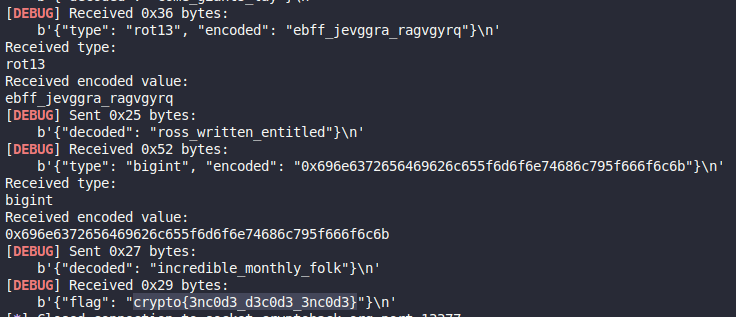
\includegraphics[width=0.8\linewidth]{Images/Encode/encode_chall_result.png}

    % La légende qui apparaîtra sous l'image.
    \caption{Capture d'écran illustrant l'obtention du \textit{flag} après le décodage 
    automatique de cent chaînes de caractères envoyées par le serveur de \textit{CryptoHack}.}

    % L'étiquette pour y faire référence plus tard.
    \label{fig:encodeChall}
\end{figure}

Le script présenté en \hyperref[annexe:script-res-encoding]{Annexe B} du rapport a permis la bonne résolution du challenge
(cf. \hyperref[fig:encodeChall]{Figure 1}) et l'obtention du \textit{flag} suivant :

\begin{center}
    \texttt{crypto\{3nc0d3\ d3c0d3\ 3nc0d3\}}
\end{center}

\subsection{XOR}

La deuxième sous-partie de la catégorie \textit{General} est consacrée à
l'opération XOR (\textit{ou} exclusif), un concept fondamental en cryptographie
constituant l'une des briques de base de nombreux algorithmes de
chiffrement. Sa simplicité de mise en œuvre et ses propriétés
mathématiques uniques en font un outil puissant pour manipuler
l'information.

Comprendre le fonctionnement du XOR est une étape cruciale, car il se
situe à la frontière entre l'opération logique et le chiffrement. L'une
de ses propriétés essentielles est sa réversibilité: appliquer deux fois
la même clé XOR à une donnée permet de retrouver la donnée originale
($A \oplus K \oplus K = A$). Cette caractéristique est au cœur de son
utilisation dans des chiffrements à flux comme le \textit{One-Time Pad}.

Nous avons décidé de présenter le challenge le plus représentatif de
cette partie, nommé \textit{Lemur XOR}.

\subsubsection{Objectifs}
Le but de ce challenge est de retrouver le \textit{flag}, à partir de
deux images fournies : \texttt{lemur.png} et \texttt{flag.png} (cf. \hyperref[fig:lemurChall]{Figure 2}). L'énoncé
nous apprend que ces deux images ont été chiffrées avec l'opération XOR en
utilisant la même clé secrète.

\begin{figure}[htbp] % L'environnement figure global
    \centering % Pour centrer le bloc des deux images

    \begin{minipage}{0.48\textwidth}
        \centering
        
\includegraphics[width=\linewidth]{Images/Lemur/flag.png}
        % Première image
    \end{minipage}
    \hfill % Ajoute un espace horizontal flexible entre les images
    \begin{minipage}{0.48\textwidth}
        \centering
        
\includegraphics[width=\linewidth]{Images/Lemur/lemur.png}
        % Deuxième image
    \end{minipage}

    \caption{Les deux images chiffrés avec une clé secrète commune. Sur la gauche \texttt{flag.png}, sur la droite \texttt{lemur.png}.}
    \label{fig:lemurChall}
\end{figure}

Le principe de résolution repose sur le fait qu'appliquer deux fois un XOR
avec la même clé annule l'opération. En effectuant un XOR entre les deux
images chiffrées que nous possédons, la clé secrète commune s'élimine,
ne laissant que le résultat du XOR entre les deux images originales.
C'est sur cette image combinée que le \textit{flag} devrait devenir
visible.

\subsubsection{Méthode}
Pour résoudre ce challenge, nous avons utilisé un script en Python avec la
bibliothèque de manipulation d'images \texttt{Pillow}. Nous avons commencé
par charger les deux images, \texttt{lemur.png} et \texttt{flag.png}.
Conformément aux instructions, nous avons appliqué l'opération XOR pixel
par pixel sur les valeurs de couleur RVB.

Nous avons donc parcouru les deux images simultanément et calculé la
nouvelle valeur de chaque pixel en effectuant un XOR sur ses composantes
rouge, verte et bleue. Nous avons ensuite utilisé ces nouveaux pixels
pour construire une image de sortie de mêmes dimensions que nous avons
sauvegardée.

\subsubsection{Résultat}

\begin{figure}[H]
    \centering
    % La commande pour insérer l'image.
    % 'width=0.8\linewidth' signifie que l'image fera 80% de la largeur du
    % texte.
    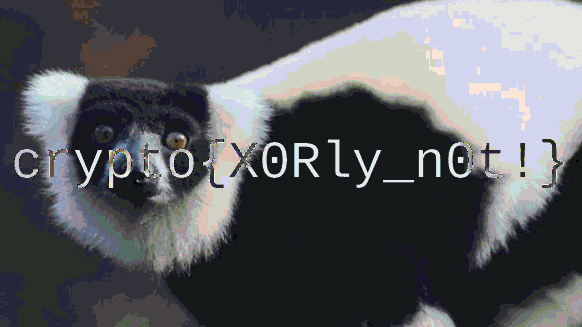
\includegraphics[width=0.8\linewidth]{Images/Lemur/xored_result.png}

    % La légende qui apparaîtra sous l'image.
    \caption{Image obtenue en effectuant un XOR pixel par pixel des deux images chiffrées.}

    % L'étiquette pour y faire référence plus tard.
    \label{fig:lemurChallRes}
\end{figure}

Le script présenté en \hyperref[annexe:script-lemur]{Annexe C} du rapport a permis la résolution du challenge en obtenant
 une image (cf. \hyperref[fig:lemurChallRes]{Figure 3}) affichant le \textit{flag} suivant :

\begin{center}
    \texttt{crypto\{X0Rly\_n0t!\}}
\end{center}


\subsection{Data formats}

Pour présenter cette gatégorie, nous avons choisi le challenge \textit{Transparency}. Pour le résoudre, nous nous appuyons sur le principe de \emph{Certificate Transparency} (CT), une mesure de sécurité imposée aux Autorités de Certification (CA) pour garantir la transparence dans la délivrance des certificats TLS.

Un certificat TLS (souvent appelé certificat SSL ou certificat numérique) remplit deux fonctions principales : il authentifie l'identité d'un site web ou d'un domaine auprès des clients (navigateurs, applications) et il permet d'établir une connexion chiffrée (TLS) entre le client et le serveur, garantissant la confidentialité et l'intégrité des données échangées.

Les \emph{CT logs} sont des bases de données publiques de type \textit{append-only} (où l'on ne peut qu'ajouter des entrées) dans lesquelles les certificats émis par les CA sont enregistrés. Aujourd'hui, les principales CA publient chaque certificat dans au moins deux logs CT publics pour qu'il soit accepté par les navigateurs modernes. Nous exploitons ces journaux pour retrouver des certificats correspondant à une clé publique donnée.

Ces logs étant audités et surveillés, nous pouvons vérifier les entrées, détecter d'éventuels certificats inattendus et contrôler la cohérence de la structure  afin de s'assurer qu'aucune entrée n'est dissimulée.

\subsubsection{Objectifs}
Nos objectifs sont doubles. D'abord, nous voulons retrouver le sous-domaine de cryptohack.org qui utilise la même clé publique que celle fournie dans le fichier \texttt{transparency.pem} au sein de son certificat TLS. Ensuite, en visitant ce sous-domaine, nous souhaitons obtenir le flag.

À travers ce challenge, nous visons d'abord à comprendre le fonctionnement d’un certificat TLS et sa structure (clé publique, signature, chaîne de confiance, etc.), ensuite de découvrir le système des \textit{Certificate Transparency logs}, puis d'apprendre à faire correspondre une clé publique à un certificat et enfin d'utiliser des outils d’investigation SSL/TLS et de recherche de certificats.

\subsubsection{Méthode}
Nous partons d'un fichier au format PEM (\textit{Privacy-Enhanced Mail}), un format standard pour les clés cryptographiques qui utilise l'encodage \textit{Base64}. La clé publique fournie est explicitée \hyperref[fig:publicKey]{Figure 4.}

\begin{figure}[H]
    \centering
\begin{lstlisting}[numbers=none]
    -----BEGIN PUBLIC KEY-----
MIIBIjANBgkqhkiG9w0BAQEFAAOCAQ8AMIIBCgKCAQEAuYj06m5q4M8SsEQwKX+5
NPs2lyB2k7geZw4rP68eUZmqODeqxDjv5mlLY2nz/RJsPdks4J+y5t96KAyo3S5g
mDqEOMG7JgoJ9KU+4HPQFzP9C8Gy+hisChdo9eF6UeWGTioazFDIdRUK+gZm81c1
iPEhOBIYu3Cau32LRtv+L9vzqre0Ollf7oeHqcbcMBIKL6MpsJMG+neJPnICI36B
ZZEMu6v6f8zIKuB7VUHAbDdQ6tsBzLpXz7XPBUeKPa1Fk8d22EI99peHwWt0RuJP
0QsJnsa4oj6C6lE+c5+vVHa6jVsZkpl2PuXZ05a69xORZ4oq+nwzK8O/St1hbNBX
sQIDAQAB
-----END PUBLIC KEY-----
\end{lstlisting}
\caption{Clé publique au format PEM fournie pour le challenge. Elle constitue le point de départ de notre recherche du certificat associé.}
    % L'étiquette pour y faire référence plus tard.
    \label{fig:publicKey}
\end{figure}

Notre méthode s'est déroulée en deux temps. Dans un premier temps, nous avons
analysé la problématique afin de comprendre comment relier l'empreinte SHA-256
d'une clé publique à un certificat TLS complet. Nous avons établi qu'un
certificat X.509 contient une clé publique et que sa représentation binaire
(DER) sert de base au calcul de l'empreinte utilisée par des services comme
\texttt{crt.sh}.

Forts de cette analyse, nous avons ensuite conçu un script Python dont les
objectifs étaient les suivants~: générer l'empreinte SHA-256 de la clé
publique fournie, interroger les journaux de transparence des certificats pour
retrouver les certificats correspondants, télécharger le certificat identifié,
en extraire le nom de domaine, et enfin y accéder pour récupérer le flag.
\subsubsection{Résultats}


Le script décrit en \hyperref[annexe:script-transparency]{Annexe D} nous a permis d'obtenir le sous-domaine recherché et d'identifier
le \textit{flag} (cf. \hyperref[tab:resultats-transparency]{Table 1}) permettant la résolution du challenge.

\begin{table}[H]
    \centering
    \renewcommand{\arraystretch}{1.5} % Augmente l'espacement vertical pour la lisibilité
    
    % On utilise tabularx pour que le tableau prenne toute la largeur du texte.
    % La première colonne est de largeur fixe (35%), la seconde (X) prend le reste.
    \begin{tabularx}{\linewidth}{| >{\bfseries}p{0.35\linewidth} | X |}
        \hline
        Empreinte (SHA-256) & \texttt{\seqsplit{29ab37df0a4e4d252f0cf12ad854bede59038fdd9cd652cbc5c222edd26d77d2}} \\ 
        \hline
        Sous-domaine identifié & \texttt{\seqsplit{thetransparencyflagishere.cryptohack.org}} \\ 
        \hline
        Flag obtenu & \texttt{crypto\{thx\_redpwn\_for\_inspiration\}} \\ 
        \hline
    \end{tabularx}
    
    \caption{Résultats obtenus pour le challenge Transparency.}
    \label{tab:resultats-transparency}
\end{table}